\documentclass[12pt, a4paper]{article}
\setlength{\headheight}{14.5pt}

\def \cname{Линейная алгебра и геометрия}
\def \pname{Экзамен 2 - 2022/2023}
\def \aname{Даниил Тимижев}
\def \hsegroup{}

\usepackage[T2A]{fontenc}
\usepackage[russian, english]{babel}
\usepackage[utf8]{inputenc}
\usepackage{subfiles}
\usepackage{ucs}
\usepackage{textcomp}
\usepackage{array}
\usepackage{indentfirst}
\usepackage{amsmath}
\usepackage{amssymb}
\usepackage{enumerate}
\usepackage[margin=1.5cm]{geometry}
\usepackage{authblk}
\usepackage{tkz-euclide}
\usepackage{icomma}
\usepackage{gensymb}
\usepackage{graphicx}
\usepackage{caption}
\usepackage{subcaption}
\usepackage{physics}
\usepackage{wrapfig}
\usepackage{tabularx, tabulary, booktabs}
\usepackage{longtable}
\usepackage{multirow}
\usepackage{xcolor}
\usepackage[unicode=true, colorlinks=true, linkcolor=blue, urlcolor=blue]{hyperref}
\usepackage{fancyhdr}
\usepackage[many]{tcolorbox}
\usepackage{mathbbol}
\usepackage{anyfontsize}

%%%%% Множества и системы %%%%%
\newcommand{\E}{\mathbb{E}}
\newcommand{\D}{\mathbb{D}}
\renewcommand{\C}{\mathbb{C}}
\newcommand{\R}{\mathbb{R}}
\newcommand{\N}{\mathbb{N}}
\newcommand{\Z}{\mathbb{Z}}
\newcommand{\Q}{\mathbb{Q}}
\newcommand{\F}{\mathbb{F}}
\newcommand{\e}{\mathbb{e}}
\renewcommand{\f}{\mathbb{f}}

%%%%% Математические обозначения %%%%%
\renewcommand{\tr}{tr}
\renewcommand{\Im}{Im}
\DeclareMathOperator{\vht}{ht}
\DeclareMathOperator{\rk}{rk}
\DeclareMathOperator{\pr}{pr}
\DeclareMathOperator{\ort}{ort}
\DeclareMathOperator{\Mat}{Mat}
\DeclareMathOperator{\vol}{vol}
\DeclareMathOperator{\Spec}{Spec}
\DeclareMathOperator{\id}{id}
\DeclareMathOperator{\Ker}{Ker}
\DeclareMathOperator{\M}{M}

%%%%% Полезности %%%%%
\renewcommand{\r}{\right}
\renewcommand{\l}{\left}
\renewcommand{\d}{\frac}
\renewcommand{\leq}{\leqslant}
\renewcommand{\geq}{\geqslant}
\newcommand{\Sum}[2]{\overset{#2}{\underset{#1}{\sum}}}
\newcommand{\Prod}[2]{\overset{#2}{\underset{#1}{\prod}}}
\newcommand{\Lim}[2]{\lim\limits_{#1 \to #2}}
\newcommand{\task}[1] {\noindent \section*{Задача №#1:}}
\newcommand{\answer}[1] {\noindent\makebox[\linewidth]{\rule{\textwidth}{0.4pt}} \subsection*{Ответ №#1:}}


%%%%% Полезные блоки %%%%%

% Расширенная матрица
\newenvironment{amatrix}[2]
{\left(\begin{array}{@{}*{#1}{c}|*{#2}{c}@{}}}
                {\end{array}\right)}

% Блок с условием
\newenvironment{condition}
{\begin{tcolorbox}[colback = green!10!white, colframe = green!75!black]}
                {\end{tcolorbox}}

% Блок с теоремой
\newenvironment{theorem}
{\begin{tcolorbox}[colback = blue!5!white, colframe = blue!75!black, opacityframe=0.2,opacityback=0.8]}
                {\end{tcolorbox}}

%%%%% Шрифт %%%%%
\renewcommand{\familydefault}{\sfdefault}

%%% Ссылки %%%
\definecolor{linkcolor}{HTML}{8b00ff}
\hypersetup{
	colorlinks = true,
	linkcolor = linkcolor,
	urlcolor = linkcolor,
	citecolor = linkcolor
}

%%% Выравнивание %%%
\setlength{\parskip}{0em}
\geometry{a4paper, left=12mm, top=25mm, right=12mm}
\setlength{\parindent}{0cm}
\linespread{1.1}

%%% Колонтитулы %%%
\pagestyle{fancy}
\fancyhf{}
\fancyhead[L]{\cname, \pname}
\fancyhead[R]{\thepage}

\title{
    \textbf{\pname}\\
    \cname
}
\author{
    \aname
    \raisebox{-3.15pt}{
        \href{https://t.me/dahbka_lis}
        {
\includegraphics[width = 16pt, height = 16pt, keepaspectratio]{source/tg_logo.png}}
    }
}
\date{\hsegroup}


\begin{document}
\maketitle
\thispagestyle{empty}

\subsection*{Введение:}
Заранее предупреждаю, что тут могут быть ошибки, поэтому никому не рекомендую полагаться на ответ, а лишь следить за ходом моих мыслей, которые я постарался описать максимально четко, вспоминая рандомные факты из курса линейной алгебры. Выражаю отдельную благодарность Александру Сидорову и Анне Зыковой, ассистентам по ЛАИГ, за помощь с разборами заданий <3.

\task{1}
\begin{condition}
    Определите все значения, которые может принимать размерность ядра линейного оператора $\varphi \colon \R^4 \to \R^4$ при условии, что в пересечении ядра и образа содержится вектор $v = (1, 2, 0, -1)$.
\end{condition}
С тем учётом, что в пересечении ядра и образа содержится вектор, смело можем утверждать, что размерность пересечения точно больше единицы:
\[
    \dim (\Ker \varphi \cap \Im \varphi) \geqslant 1
\]

Теперь оценим размерность ядра $\varphi$:
\[
    1 \leqslant \dim(\Ker \varphi \cap \Im \varphi) \leqslant \dim \Ker \varphi \leqslant \dim(\Ker \varphi + \Im \varphi) \leqslant 4 = \dim \R^4
\]

Отметим тот факт, что вектор $v$ лежит также в образе $\varphi$, с чего делаем вывод, что и размерность $\Im \varphi$ ненулевая. Тогда воспользуемся \textit{теоремой о связи размерностей ядра и образа линейного отображения}:
\begin{theorem}
    \[
        \dim \Im \varphi + \dim \Ker \varphi = \dim V
    \]
\end{theorem}

В нашем же случае $\dim \Ker \varphi + \dim \Im \varphi = \dim \R^4 = 4$, тогда понятно, что $\dim \Ker \varphi \in \{1, 2, 3\}$. Рассмотрим каждый случай и приведём примеры \textbf{(без примеров потеря баллов)}. Для каждого примера дополняем вектор $v$ векторами стандартного базиса $\R^4$, назовём базис $\e = (v, e_1, e_2, e_3)$:

\begin{enumerate}
    \item $\dim \Ker \varphi = 1$:{
          В таком случае можем построить отображение, которое переводит лишь вектор $v$ в нулевой. Матрица оператора будет иметь следующий вид в нашем базисе:
          \[
              A(\varphi, \e) =
              \begin{pmatrix}
                  0 & 1 & 0 & 0 \\
                  0 & 0 & 1 & 0 \\
                  0 & 0 & 0 & 1 \\
                  0 & 0 & 0 & 0
              \end{pmatrix}
              \implies
              \begin{cases}
                  v \to \vec{0} \\
                  e_1 \to v     \\
                  e_2 \to e_1   \\
                  e_3 \to e_2
              \end{cases}
          \]
          }

    \item $\dim \Ker \varphi = 2$:{
          В таком случае можем построить отображение, которое переводит векторы $v$ и $e_1$ в нулевой. Матрица оператора будет иметь следующий вид в нашем базисе:
          \[
              A(\varphi, \e) =
              \begin{pmatrix}
                  0 & 0 & 1 & 0 \\
                  0 & 0 & 0 & 0 \\
                  0 & 0 & 0 & 1 \\
                  0 & 0 & 0 & 0
              \end{pmatrix}
              \implies
              \begin{cases}
                  v, e_1 \to \vec{0} \\
                  e_2 \to v          \\
                  e_3 \to e_2
              \end{cases}
          \]
          }

    \item $\dim \Ker \varphi = 3$:{
          В таком случае можем построить отображение, которое переводит векторы $v$, $e_1$ и $e_2$ в нулевой. Матрица оператора будет иметь следующий вид в нашем базисе:
          \[
              A(\varphi, \e) =
              \begin{pmatrix}
                  0 & 0 & 0 & 1 \\
                  0 & 0 & 0 & 0 \\
                  0 & 0 & 0 & 0 \\
                  0 & 0 & 0 & 0
              \end{pmatrix}
              \implies
              \begin{cases}
                  v, e_1, e_2 \to \vec{0} \\
                  e_3 \to v
              \end{cases}
          \]
          }
\end{enumerate}

\answer{1}
Размерность ядра линейного оператора $\varphi$ может принимать значения от 1 до 3. Примеры приведены выше.

\newpage
\task{2}
\begin{condition}
    Приведите пример неопределённой квадратичной формы $Q \colon \R^3 \to \R$, принимающей отрицательные значения на всех ненулевых векторах подпространства:
    \[
        \{ (x, y, z) \in \R^3 \mid x - 2y + z = 0 \}
    \]
    Ответ представьте в стандартном виде многочлена 2-й степени от координат $x,y,z$.
\end{condition}

Пусть $S = \{ (x, y, z) \in \R^3 \mid x - 2y + z = 0 \}$. Тогда $S$ - подпространство решений ОСЛУ. Найдём базис через ФСР:
\[
    x - 2y + z = 0
    \implies
    \begin{amatrix}{3}{1}
        1 & -2 & 1 & 0
    \end{amatrix}
    \leadsto
    S =
    \langle
    \underbrace{
        \begin{pmatrix}
            -1 \\
            0  \\
            1
        \end{pmatrix}
    }_{f_1}, \;
    \underbrace{
        \begin{pmatrix}
            2 \\
            1 \\
            0
        \end{pmatrix}
    }_{f_2}
    \rangle
\]

Зададим квадратичную форму $Q$ так, чтобы $Q(S) < 0$. В таком случае векторы $f_1, f_2$ отобразим в отрицательные значения. Так как $Q$ задаём на $\R^3$ по условию, дополним базис $S$ до базиса всего пространства:
\[
    f_3 =
    \begin{pmatrix}
        0 \\
        0 \\
        1
    \end{pmatrix},
    \quad
    \begin{pmatrix}
        f_1 & f_2 & f_3
    \end{pmatrix}
    =
    \begin{pmatrix}
        -1 & 2 & 0 \\
        0  & 1 & 0 \\
        1  & 0 & 1
    \end{pmatrix}
    \leadsto
    \begin{pmatrix}
        1 & 0 & 0 \\
        0 & 1 & 0 \\
        0 & 0 & 1
    \end{pmatrix}
    \implies
    \f = (f_1, f_2, f_3) \text{ - базис в } \R^3
\]

\begin{theorem}
    $Q$ - неопределённая, если её индексы инерции $i_+, i_-$ равны некоторым ненулевым значениям.
\end{theorem}

Пусть значение квадратичной формы $Q$ отрицательно для $f_1, f_2$ (векторы базиса $S$), а для $f_3$ - положительно, тогда в базисе $\f$ она будет иметь нормальный вид с такой матрицей:
\[
    B(Q, \f) =
    \begin{pmatrix}
        -1 & 0  & 0 \\
        0  & -1 & 0 \\
        0  & 0  & 1
    \end{pmatrix},
    \quad
    \begin{cases}
        i_+ = 1 \\
        i_- = 2
    \end{cases}
\]

Мы задали неопределённую квадратичную форму в нормальном виде. Найдём её исходный вид, вспомнив \textit{Закон инерции}:

\begin{theorem}
    Числа $i_+$ и $i_-$ не зависят от выбора базиса, в котором $Q$ принимает нормальный вид.
\end{theorem}

В таком неопределённость нашей квадратичной формы $Q$ останется на месте при смене базиса.

Пусть $\e$ - базис, в котором $Q$ имеет стандартный вид, причём $\f = \e \cdot C$, где $C$ - матрица перехода. Полагаем, что $\e$ - стандартный базис, тогда соберём $C$ из векторов базиса $\f$:
\[
    C =
    \begin{pmatrix}
        -1 & 2 & 0 \\
        0  & 1 & 0 \\
        1  & 0 & 1
    \end{pmatrix}
\]

\newpage

Далее, для нахождения матрицы стандартного вида $Q$ рассмотрим формулу смены базиса квадратичной формы в терминах базисов $\f$ и $\e$:
\[
    B(Q, \f) = C^T \cdot B(Q, \e) \cdot C
    \;
    \implies
    \;
    B(Q, \e) = (C^{-1})^T \cdot B(Q, \f) \cdot C^{-1}
\]

Воспользуемся методом Гаусса для нахождения $C^{-1}$:
\[
    (C \mid E) =
    \begin{amatrix}{3}{3}
        -1 & 2 & 0 & 1 & 0 & 0 \\
        0 & 1 & 0 & 0 & 1 & 0 \\
        1 & 0 & 1 & 0 & 0 & 1
    \end{amatrix}
    \leadsto
    \begin{amatrix}{3}{3}
        1 & 0 & 0 & -1 & 2 & 0 \\
        0 & 1 & 0 & 0 & 1 & 0 \\
        0 & 0 & 1 & 1 & -2 & 1
    \end{amatrix}
    =
    (E \mid C^{-1})
\]

Найдем матрицу квадратичной формы $Q$ в базисе $\e$:
\[
    B(Q, \e) =
    \begin{pmatrix}
        -1 & 2  & 0 \\
        0  & 1  & 0 \\
        1  & -2 & 1
    \end{pmatrix}^T
    \begin{pmatrix}
        -1 & 0  & 0 \\
        0  & -1 & 0 \\
        0  & 0  & 1
    \end{pmatrix}
    \begin{pmatrix}
        -1 & 2  & 0 \\
        0  & 1  & 0 \\
        1  & -2 & 1
    \end{pmatrix}
    =
    \begin{pmatrix}
        0 & 0  & 1  \\
        0 & -1 & -2 \\
        1 & -2 & 1
    \end{pmatrix}
\]

Пусть $X = (x \; y \; z)$. Тогда по $B(Q, \e)$ выпишем стандартный вид квадратичной формы $Q$ от координат $x, y, z$:
\[
    Q(X) = 2xz - y^2 - 4yz + z^2
\]

\answer{2}
Пример подходящей квадратичной формы: $Q(X) = 2xz - y^2 - 4yz + z^2$.

\newpage
\task{3}
\begin{condition}
    В евклидовом пространстве $\R^3$ со стандартным скалярным произведением даны векторы:
    \[
        u_1 = (-1, 1, 2), \;
        u_2 = (1, 1, -1), \;
        u_3 = (1, -1, 0)
    \]
    Обозначим через $v_1, v_2, v_3$ ортогональные проекции вектора $v = (3, -5, 1)$ на подпространства $u_1^\bot, u_2^\bot, u_3^\bot$ соответственно. Найдите объем параллелепипеда, натянутого на векторы $v_1, v_2, v_3$.
\end{condition}

Для нахождения векторов $v_1, v_2, v_3$ в явном виде воспользуемся таким фактом:
\begin{theorem}
    \[
        \forall \; u, v \in \E \colon \pr_u v = \ort_{u^\bot} v, \; \ort_u v = \pr_{u^\bot} v
    \]
\end{theorem}

Выпишем векторы, заданные условием:
\begin{itemize}
    \item $v_1 = \pr_{u_1^\bot} v = \ort_{u_1} v = v - \pr_{u_1} v = v - \d{(v, u_1)}{(u_1, u_1)} u_1 = v + u_1 = (2, -4, 3)$

    \item $v_2 = \pr_{u_2^\bot} v = \ort_{u_2} v = v - \pr_{u_2} v = v - \d{(v, u_2)}{(u_2, u_2)} u_2 = v + u_2 = (4, -4, 0)$

    \item $v_3 = \pr_{u_3^\bot} v = \ort_{u_3} v = v - \pr_{u_3} v = v - \d{(v, u_3)}{(u_3, u_3)} u_3 = v - 4 u_3 = (-1, -1, 1)$
\end{itemize}

Существует много различных способов найти объем параллелепипеда, я воспользуюсь вычислением через матрицу Грама:
\begin{theorem}
    \[
        \vol P(v_1, v_2, v_3)^2 = \det G(v_1, v_2, v_3)
    \]
\end{theorem}

Соберём матрицу Грама явно:
\[
    G := G(v_1, v_2, v_3)
    =
    \begin{pmatrix}
        (v_1, v_1) & (v_1, v_2) & (v_1, v_3) \\
        (v_2, v_1) & (v_2, v_2) & (v_2, v_3) \\
        (v_3, v_1) & (v_3, v_2) & (v_3, v_3)
    \end{pmatrix}
    =
    \begin{pmatrix}
        29 & 24 & 5 \\
        24 & 32 & 0 \\
        5  & 0  & 3
    \end{pmatrix}
\]

Найдём определитель для $G$:
\[
    \det G =
    29 \cdot 32 \cdot 3 + 0 + 0 - 5 \cdot 5 \cdot 32 - 0 - 24 \cdot 24 \cdot 3 = 2784 - 800 - 1728 = 256
\]

Тогда $\vol P(v_1, v_2, v_3)^2 = \det G = 256$, получаем $\vol P(v_1, v_2, v_3) = \sqrt{256} = 16$.

\answer{3}
Объем параллелепипеда, натянутого на векторы $v_1, v_2, v_3$, равен 16.

\newpage
\task{4}
\begin{condition}
    Приведите пример недиагонализуемого линейного оператора $\varphi$ в $\R^2$, для которого оператор
    \mbox{$\varphi^2 - 5 \varphi$} диагонализуем.
\end{condition}

Зададим $\varphi \colon \R^2 \to \R^2$ - линейный оператор с матрицей $A := A(\varphi, \e)$ в некотором базисе $\e$. $\varphi$ недиагонализуем, тогда пусть матрица $A$ имеет жорданову нормальную форму:
\[
    A =
    \begin{pmatrix}
        x & 1 \\
        0 & x
    \end{pmatrix},
    \quad
    x \in \Spec \varphi
\]

\begin{theorem}
    Пусть $V$ - векторное пространство над полем $F$. Тогда $\forall \; \varphi, \psi \in L(V), \;\lambda \in F$ в некотором базисе $\e$ имеем:
    \[
        A(\varphi \circ \psi, \e) = A(\varphi, \e) \cdot A(\psi, \e),
        \quad
        A(\lambda \varphi, \e) = \lambda \cdot A(\varphi, \e)
    \]
\end{theorem}

Вычислим явно, чему будет равна матрица оператора $\varphi^2 - 5 \varphi$:
\[
    A(\varphi^2 - 5 \varphi, \e) = A^2 - 5A =
    \begin{pmatrix}
        x^2 & 2x  \\
        0   & x^2
    \end{pmatrix}
    -
    \begin{pmatrix}
        5x & 5  \\
        0  & 5x
    \end{pmatrix}
    =
    \begin{pmatrix}
        x(x - 5) & 2x - 5   \\
        0        & x(x - 5)
    \end{pmatrix}
\]

Заметим, что $\varphi^2 - 5 \varphi$ диагонализуем, если $2x - 5 = 0$ (так как матрица уже будет иметь диагональный вид). Тогда нам подойдёт значение $x = \d{5}{2}$:
\[
    A(\varphi^2 - 5 \varphi, \e) =
    \begin{pmatrix}
        x(x - 5) & 2x - 5   \\
        0        & x(x - 5)
    \end{pmatrix}
    =
    \begin{pmatrix}
        -\d{25}{4} & 0          \\
        0          & -\d{25}{4}
    \end{pmatrix}
\]

Подставим значение в матрицу $A$:
\[
    A =
    \begin{pmatrix}
        \d{5}{2} & 1        \\
        0        & \d{5}{2}
    \end{pmatrix}
    \text{ - ЖНФ}
\]

\answer{4}
Линейный оператор $\varphi \colon \R^2 \to \R^2$, задаваемый матрицей:
\[
    A(\varphi, \e) =
    \begin{pmatrix}
        \d{5}{2} & 1        \\
        0        & \d{5}{2}
    \end{pmatrix}
\]

\newpage
\task{5}
\begin{condition}
    Вставьте вместо звёздочки, ромбика и кружочка подходящие числа таким образом, чтобы линейный оператор $\varphi \colon \R^3 \to \R^3$, имеющий в стандартном базисе матрицу:
    \[
        \begin{pmatrix}
            2/3      & *    & 2/3   \\
            -1/3     & -2/3 & 2/3   \\
            \diamond & 2/3  & \circ
        \end{pmatrix},
    \]
    был ортогональным. Найдите ортонормированный базис, в котором матрица оператора $\varphi$ имеет канонический вид и выпишите эту матрицу. Укажите ось и угол поворота, определяемого оператором $\varphi$.
\end{condition}

Для начала разберёмся с неизвестными значениями. Знаем, что матрица ортогонального оператора является \textit{ортогональной} (столбцы/строки матрицы образуют ортонормированную систему).
\[
    A := A(\varphi, \e)
    =
    \begin{pmatrix}
        2/3      & *    & 2/3   \\
        -1/3     & -2/3 & 2/3   \\
        \diamond & 2/3  & \circ
    \end{pmatrix}
\]

Найдём значения, при которых длины столбцов матрицы $A$ равны 1:
\begin{itemize}
    \item $(A^{(1)}, A^{(1)}) = \d{4}{9} + \d{1}{9} + \diamond^2 = 1 \implies \diamond = \pm \d{2}{3}$

    \item $(A^{(2)}, A^{(2)}) = *^2 + \d{4}{9} + \d{4}{9} = 1 \implies * = \pm \d{1}{3}$

    \item $(A^{(3)}, A^{(3)}) = \d{4}{9} + \d{4}{9} + \circ^2 = 1 \implies \circ = \pm \d{1}{3}$
\end{itemize}

Система векторов называется ортогональной, если попарное скалярное произведение векторов из системы равно нулю. Методом перебора понимаем, что нам подходят такие значения:
\[
    \diamond = -\d{2}{3},
    \quad
    * = \d{1}{3},
    \quad
    \circ = \d{1}{3}
\]

Тогда, перед нами матрица ортогонального оператора $\varphi$:
\[
    A =
    \begin{pmatrix}
        2/3  & 1/3  & 2/3 \\
        -1/3 & -2/3 & 2/3 \\
        -2/3 & 2/3  & 1/3
    \end{pmatrix}
\]

\begin{theorem}
    Классификация ортогональных операторов в трёхмерном евклидовом пространстве:
    \[
        \exists \; \e \text{ - ОНБ } \colon
        A(\varphi, \e) =
        \begin{pmatrix}
            \cos{\alpha} & -\sin{\alpha} & 0    \\
            \sin{\alpha} & \cos{\alpha}  & 0    \\
            0            & 0             & \pm1
        \end{pmatrix}
    \]
\end{theorem}

\textit{Примечательный факт}: $\Spec \varphi$, где $\varphi$ - ортогональный линейный оператор, всегда хранит в себе значение 1 или -1 в случае $\R^3$.

\newpage

Посчитаем характеристический многочлен, дабы удостовериться в этом. Можно сразу же искать вектор, за выбрав собственное значение 1 или -1 (и надеяться, что оно подойдёт):
\[
    \chi_t(\varphi) = (-1)^3 \det(A - tE) = \d{3t^3 - t^2 - t + 3}{3} = \d{1}{3}(t + 1)(3t^2 - 4t + 3) \implies -1 \in \Spec \varphi
\]

Найдём базис для собственного подпространства $V_{-1}(\varphi)$ через ФСР:
\[
    (A - (-1) \cdot E) = (A + E) =
    \begin{pmatrix}
        5/3  & 1/3 & 2/3 \\
        -1/3 & 1/3 & 2/3 \\
        -2/3 & 2/3 & 4/3
    \end{pmatrix}
    \leadsto
    \begin{pmatrix}
        1 & 0 & 0 \\
        0 & 1 & 2 \\
        0 & 0 & 0
    \end{pmatrix}
    \implies e_3 =
    \begin{pmatrix}
        0  \\
        -2 \\
        1
    \end{pmatrix}
\]

Вектор $e_3$ находится в искомом базисе. Оставшиеся векторы $e_1, e_2$ найдём как $\langle e_3 \rangle^\bot = \langle e_1, e_2 \rangle$ через ФСР:
\[
    (e_3) =
    \begin{pmatrix}
        0 & -2 & 1
    \end{pmatrix}
    \leadsto
    e_1 =
    \begin{pmatrix}
        1 \\
        0 \\
        0
    \end{pmatrix}, \;
    e_2 =
    \begin{pmatrix}
        0   \\
        1/2 \\
        1
    \end{pmatrix}
\]

Заметим, что $e_1, e_2$ - ортогональны друг другу (в ином случае потребовалось бы ортогонализовать), тогда система $(e_1, e_2, e_3)$ является ортогональной. Нормируем:
\begin{itemize}
    \item $f_1 = \d{1}{|e_1|} e_1 = e_1 = (1, 0, 0)$

    \item $f_2 = \d{1}{|e_2|} e_2 = \d{2\sqrt{5}}{5} e_2 =
              \l(0,\; \d{\sqrt{5}}{5},\; \d{2 \sqrt{5}}{5}\r)$

    \item $f_3 = \d{1}{|e_3|} e_3 =\d{\sqrt{5}}{5} e_3 =
              \l(0,\; -\d{2 \sqrt{5}}{5},\; \d{\sqrt{5}}{5}\r)$
\end{itemize}

Получаем систему $\f = (f_1, f_2, f_3)$ - ортонормированный базис, в котором матрица ортогонального оператора имеет канонический вид.

\begin{theorem}
    \[
        \cos{\alpha} = (\varphi(f_1), f_1),
        \quad
        \sin{\alpha} = (\varphi(f_1), f_2)
    \]
\end{theorem}

Найдём $\varphi(f_1)$:
\[
    \varphi(f_1) = A f_1 =
    \begin{pmatrix}
        2/3  & 1/3  & 2/3 \\
        -1/3 & -2/3 & 2/3 \\
        -2/3 & 2/3  & 1/3
    \end{pmatrix}
    \begin{pmatrix}
        1 \\
        0 \\
        0
    \end{pmatrix}
    =
    \begin{pmatrix}
        2/3  \\
        -1/3 \\
        -2/3
    \end{pmatrix}
\]
Теперь вычислим значения $\cos{\alpha}$ и $\sin{\alpha}$:
\begin{itemize}
    \item $\cos{\alpha} = (\varphi(f_1), f_1) = \frac{2}{3}$.

    \item $\sin{\alpha} = (\varphi(f_1), f_2) = -\d{\sqrt{5}}{15} - \d{4 \sqrt{5}}{15} = -\d{\sqrt{5}}{3}$
\end{itemize}

\newpage

Итого, в базисе $\f$ матрица оператора $\varphi$ имеет такой канонический вид:
\[
    A(\varphi, \f) =
    \begin{pmatrix}
        2/3         & \sqrt{5}/3 & 0  \\
        -\sqrt{5}/3 & 2/3        & 0  \\
        0           & 0          & -1
    \end{pmatrix}
\]

Данная матрица является матрицей поворота вокруг вектора $f_3$ на угол $\arccos{\frac{2}{3}}$ с зеркальным отражением.

\answer{5}
\begin{itemize}
    \item Базис
          $
              \f =
              (
              \begin{pmatrix}
                  1 \\[1mm]
                  0 \\[1mm]
                  0
              \end{pmatrix}, \;
              \begin{pmatrix}
                  0               \\[1mm]
                  \d{\sqrt{5}}{5} \\[1mm]
                  \d{2 \sqrt{5}}{5}
              \end{pmatrix}, \;
              \begin{pmatrix}
                  0                  \\[1mm]
                  -\d{2 \sqrt{5}}{5} \\[1mm]
                  \d{\sqrt{5}}{5}
              \end{pmatrix}
              )
          $.

    \item Канонический вид:
          $
              A(\varphi, \f)
              =
              \begin{pmatrix}
                  2/3         & \sqrt{5}/3 & 0  \\
                  -\sqrt{5}/3 & 2/3        & 0  \\
                  0           & 0          & -1
              \end{pmatrix}
          $.

    \item Поворот вокруг вектора $\l(0,\; -\d{2 \sqrt{5}}{5},\; \d{\sqrt{5}}{5}\r)$ на угол $\arccos{\d{2}{3}}$ и зеркальное отражение.
\end{itemize}

\newpage
\task{6}
\begin{condition}
    Существует ли матрица $A \in \Mat_{2 \times 3}(\R)$ ранга 2 со следующими свойствами:
    \begin{enumerate}
        \item[1)] одно из сингулярных значений матрицы $A$ равно $\sqrt{20}$;

        \item[2)] ближайшая к $A$ по норме Фробениуса матрица ранга $1$ есть
            $
                B =
                \begin{pmatrix}
                    3 & -3 & 3 \\
                    1 & -1 & 1
                \end{pmatrix}
            $?
    \end{enumerate}
    Если существует, то предъявите такую матрицу.
\end{condition}

Рассмотрим теоретическое сингулярное разложение матрицы $A$. Пусть:
\[
    A = U \cdot \Sigma \cdot V^T
\]
где $U = (u_1 \ \; u_2),\; V^T = (v_1 \ \; v_2 \ \; v_3)$ и $\Sigma =
    \begin{pmatrix}
        \sigma_1 & 0        & 0 \\
        0        & \sigma_2 & 0
    \end{pmatrix}$, причём $u_1, u_2 \in \R^2$ и $v_1, v_2, v_3 \in \R^3$.
\\[5mm]
Вспомним предложение с лекции:
\[
    A = U \cdot \Sigma \cdot V^T = u_1 \sigma_1 v_1^T + u_2 \sigma_2 v_2^T
\]
Рассмотрим теорему о низкоранговом приближении:
\begin{theorem}
    Пусть $A \in \Mat_{m \times n}(\R), \; \rk A = r$. Пусть $A = U \Sigma V^T$ - SVD для $A$. $\forall \; k = 1, \; \ldots, \; r - 1 $ положим:
    \[
        \Sigma_k =
        \begin{pmatrix}
            \sigma_1 & \cdots & 0        & \cdots & 0      \\
            \vdots   & \ddots & \vdots   & \ddots & \vdots \\
            0        & \cdots & \sigma_k & \cdots & 0      \\
            \vdots   & \ddots & \vdots   & \ddots & \vdots \\
            0        & \cdots & 0        & \cdots & 0
        \end{pmatrix}
        \text{ - первые $k$ сингулярных значений}
    \]
    Тогда минимум величины $\Vert A - B \Vert$ (норма Фробениуса) среди всех матриц $B$ ранга $\leq k$ достигается при $B = U \Sigma_k V^T$.
\end{theorem}

По теореме понимаем, что матрица $B$ ранга 1 максимально приближает неизвестную матрицу $A$, если $B = U \Sigma_1 V^T$. Тогда $\Sigma_1 = \sigma_1$ и, соответственно, $B = u_1 \sigma_1 v_1^T$.

Заметим, что:
\[
    B =
    \begin{pmatrix}
        3 & -3 & 3 \\
        1 & -1 & 1
    \end{pmatrix}
    =
    \begin{pmatrix}
        3 \\
        1
    \end{pmatrix}
    \begin{pmatrix}
        1 & -1 & 1
    \end{pmatrix}
\]
Нормируем векторы и получим:
\[
    B =
    \begin{pmatrix}
        3 \\
        1
    \end{pmatrix}
    \begin{pmatrix}
        1 & -1 & 1
    \end{pmatrix}
    =
    \sqrt{10}
    \begin{pmatrix}
        \d{3 \sqrt{10}}{10} \\[0.7mm]
        \d{\sqrt{10}}{10}
    \end{pmatrix}
    \cdot
    \sqrt{3}
    \begin{pmatrix}
        \d{\sqrt{3}}{3} & -\d{\sqrt{3}}{3} & \d{\sqrt{3}}{3}
    \end{pmatrix}
    =
    \underbrace{
        \begin{pmatrix}
            \d{3 \sqrt{10}}{10} \\[0.7mm]
            \d{\sqrt{10}}{10}
        \end{pmatrix}
    }_{u_1}
    \underbrace{\sqrt{30}}_{\sigma_1}
    \underbrace{
        \begin{pmatrix}
            \d{\sqrt{3}}{3} & -\d{\sqrt{3}}{3} & \d{\sqrt{3}}{3}
        \end{pmatrix}
    }_{v_1^T}
\]
Таким образом, мы получили первую компоненту ранга 1 для сингулярного разложения матрицы $A$. Далее, по условию задачи полагаем $\sigma_2 = \sqrt{20}$. Заметим, что $\sigma_1 = \sqrt{30} > \sigma_2 = \sqrt{20}$, значит разложение определено верно. Тогда имеем:
\[
    A = u_1 \sqrt{30}\  v_1^T + u_2 \sqrt{20}\  v_2^T
\]

Придумаем, каким образом мы можем при нормировке получить $\sigma_2 = \sqrt{20}$. В первом случае из вектора $u_1$ мы вынесли $\sqrt{10}$, из $v_1$ получили $\sqrt{3}$. Тогда за $u_2$ возьмём и нормируем такой вектор, который является ортогональным относительно $u_1$ и его длина равна $\sqrt{10}$. Например:
\[
    \begin{pmatrix}
        -1 \\
        3
    \end{pmatrix}
    \implies
    u_2 =
    \frac{1}{\sqrt{10}}
    \begin{pmatrix}
        -1 \\
        3
    \end{pmatrix}, \quad
    (u_1,\; u_2) = -3 + 3 = 0
\]
Теперь для $v_2$ подберём такой вектор, который является ортогональным к $v_1$ и с длиной $\sqrt{2}$ (так как $\sqrt{20} = \sqrt{10} \cdot \sqrt{2}$, а $\sqrt{10}$ из вектора $u_2$). Если посмотреть на $v_1$ до нормировки, сразу приходят на ум такие ортогональные к нему векторы:
\[
    \{
    \begin{pmatrix}
        1 \\
        1 \\
        0
    \end{pmatrix},\;
    \begin{pmatrix}
        0 \\
        1 \\
        1 \\
    \end{pmatrix},\;
    \begin{pmatrix}
        \pm 1 \\
        0     \\
        \mp 1
    \end{pmatrix}
    \}
\]
Возьмём первый вектор, тогда имеем:
\[
    \begin{pmatrix}
        1 \\
        1 \\
        0
    \end{pmatrix}
    \implies
    v_2 = \d{1}{\sqrt{2}}
    \begin{pmatrix}
        1 \\
        1 \\
        0
    \end{pmatrix}, \quad
    (v_1, \;v_2) = \d{\sqrt{6}}{6} - \d{\sqrt{6}}{6} = 0
\]
Итого, наборы $(u_1, u_2)$ и $(v_1, v_2)$ являются ортонормированными системами. Найдём матрицу $A$:
\[
    A = u_1 \sqrt{30}\  v_1^T + u_2 \sqrt{20}\  v_2^T =
    \begin{pmatrix}
        \d{3 \sqrt{10}}{10} \\[0.7mm]
        \d{\sqrt{10}}{10}
    \end{pmatrix}
    \sqrt{30}
    \begin{pmatrix}
        \d{\sqrt{3}}{3} & -\d{\sqrt{3}}{3} & \d{\sqrt{3}}{3}
    \end{pmatrix}
    +
    \begin{pmatrix}
        -\d{\sqrt{10}}{10} \\[0.7mm]
        \d{3 \sqrt{10}}{10}
    \end{pmatrix}
    \sqrt{20}
    \begin{pmatrix}
        \d{\sqrt{2}}{2} & \d{\sqrt{2}}{2}
    \end{pmatrix}
    =
\]
\[
    =
    \begin{pmatrix}
        3 \\
        1
    \end{pmatrix}
    \begin{pmatrix}
        1 & -1 & 1
    \end{pmatrix}
    +
    \begin{pmatrix}
        -1 \\
        3
    \end{pmatrix}
    \begin{pmatrix}
        1 & 1 & 0
    \end{pmatrix}
    =
    \begin{pmatrix}
        3 & -3 & 3 \\
        1 & -1 & 1
    \end{pmatrix}
    +
    \begin{pmatrix}
        -1 & -1 & 0 \\
        3  & 3  & 0
    \end{pmatrix}
    =
    \begin{pmatrix}
        2 & -4 & 3 \\
        4 & 2  & 1
    \end{pmatrix}
\]

\answer{6}
Да, существует:
$
    A =
    \begin{pmatrix}
        2 & -4 & 3 \\
        4 & 2  & 1
    \end{pmatrix}
    =
    U \Sigma V^T
$, где
$
    \Sigma =
    \begin{pmatrix}
        \sqrt{30} & 0         & 0 \\
        0         & \sqrt{20} & 0 \\
    \end{pmatrix}
$.

\newpage
\task{7}
\begin{condition}
    Найдите прямоугольную декартову систему координат в $\R^3$ (выражение старых координат через новые), в которой уравнение поверхности
    \[
        2y^2 - 3z^2 + 4xz - 8y + 5 = 0
    \]
    имеет канонический вид. Укажите этот вид, определите тип поверхности и нарисуйте её эскиз.
\end{condition}

Рассмотрим данное уравнение как некоторую квадратичную форму. Далее, для получения канонического вида нам поможет \textit{теорема о приведении квадратичной формы к главным осям}:

\begin{theorem}
    Для любой квадратичной формы $Q \colon \E \to \R$ существует ортонормированный базис $\e = (e_1, \ldots, e_n)$, в котором $Q$ принимает канонический вид $Q(x) = \lambda_1 x_1^2 + \ldots + \lambda_n x_n^2$. Более того, набор $\lambda_1, \ldots, \lambda_n$ определён однозначно с точностью до перестановки.
\end{theorem}

Перепишем квадратичную форму как матрицу, последние слагаемые $(- 8y + 5)$ подставим после приведения:
\[
    Q(x, y, z) = 2y^2 - 3z^2 + 4xz
    \implies
    B(Q, \e) =
    \begin{pmatrix}
        0 & 0 & 2  \\
        0 & 2 & 0  \\
        2 & 0 & -3
    \end{pmatrix}
\]

Нетрудно заметить, что вышеописанная теорема работает за счёт симметричности матрицы квадратичной формы, а ведь симметричные матрицы всегда диагонализуемы, требуется лишь вычислить ортонормированный базис из собственных векторов. Найдём спектр:
\[
    \chi_B(t) = (-1)^n \det(B -tE) = -
    \begin{vmatrix}
        -t & 0     & 2      \\
        0  & 2 - t &        \\
        2  & 0     & -3 - t
    \end{vmatrix}
    = (t - 2)(t + 4)(t - 1) \implies \Spec B = \{1, 2, -4\}
\]

Теперь вычислим базис из собственных векторов:
\begin{enumerate}
    \item $\lambda = 2:$
          \[
              B - 2E =
              \begin{pmatrix}
                  -2 & 0 & 2  \\
                  0  & 0 & 0  \\
                  2  & 0 & -5
              \end{pmatrix}
              \leadsto
              \begin{pmatrix}
                  1 & 0 & 0 \\
                  0 & 0 & 1 \\
                  0 & 0 & 0
              \end{pmatrix}
              \implies
              u_1 =
              \begin{pmatrix}
                  0 \\
                  1 \\
                  0
              \end{pmatrix}
          \]

    \item $\lambda = -4:$
          \[
              B + 4E =
              \begin{pmatrix}
                  4 & 0 & 2 \\
                  0 & 6 & 0 \\
                  2 & 0 & 1
              \end{pmatrix}
              \leadsto
              \begin{pmatrix}
                  1 & 0 & \d{1}{2} \\
                  0 & 1 & 0        \\
                  0 & 0 & 0
              \end{pmatrix}
              \implies
              u_2 =
              \begin{pmatrix}
                  -\d{1}{2} \\
                  0         \\
                  1
              \end{pmatrix}
          \]

    \item $\lambda = 1:$
          \[
              B - E =
              \begin{pmatrix}
                  -1 & 0 & 2  \\
                  0  & 1 & 0  \\
                  2  & 0 & -4
              \end{pmatrix}
              \leadsto
              \begin{pmatrix}
                  1 & 0 & -2 \\
                  0 & 1 & 0  \\
                  0 & 0 & 0
              \end{pmatrix}
              \implies
              u_3 =
              \begin{pmatrix}
                  2 \\
                  0 \\
                  1
              \end{pmatrix}
          \]
\end{enumerate}

Полученные векторы ортонормируем $\f = \l( \d{u_1}{|u_1|}, \d{u_2}{|u_2|}, \d{u_3}{|u_3|} \r)$:

\newpage

\[
    f_1 = \d{u_1}{|u_1|} =
    \begin{pmatrix}
        0 \\
        1 \\
        0
    \end{pmatrix},
    \quad
    f_2 = \d{u_2}{|u_2|} =
    \begin{pmatrix}
        -\d{1}{\sqrt{5}} \\
        0                \\
        \d{2}{\sqrt{5}}
    \end{pmatrix},
    \quad
    f_3 = \d{u_3}{|u_3|} =
    \begin{pmatrix}
        \d{2}{\sqrt{5}} \\
        0               \\
        \d{1}{\sqrt{5}}
    \end{pmatrix}
\]

Собираем полученные векторы в матрицу и получаем такую замену координат:
\[
    \begin{pmatrix}
        x \\
        y \\
        z
    \end{pmatrix}
    =
    \begin{pmatrix}
        0 & -\d{1}{\sqrt{5}} & \d{2}{\sqrt{5}} \\
        1 & 0                & 0               \\
        0 & \d{2}{\sqrt{5}}  & \d{1}{\sqrt{5}}
    \end{pmatrix}
    \begin{pmatrix}
        x' \\
        y' \\
        z'
    \end{pmatrix}
    \iff
    \begin{cases}
        x = -\d{1}{\sqrt{5}} y' + \d{2}{\sqrt{5}} z' \\
        y = x'                                       \\
        z = \d{2}{\sqrt{5}} y' + \d{1}{\sqrt{5}} z'
    \end{cases}
\]

Получим такое уравнение:
\[
    2y^2 - 3z^2 + 4xz - 8y + 5 = 0 \implies 2{x'}^2 - 4{y'}^2 + {z'}^2 - 8x' + 5 = 0
\]

Теперь соберём оставшиеся слагаемые, чтобы получить канонический вид полностью:
\[
    2{x'}^2 - 4{y'}^2 + {z'}^2 - 8x' + 5
    \implies
    2({x'}^2 - 4x' + 4) - 8 - 4{y'}^2 + {z'}^2 + 5 \implies
\]
\[
    \implies
    2(x' - 2)^2 - 4{y'}^2 + {z'}^2 - 3 = 0
    \implies
    2(x' - 2)^2 - 4{y'}^2 + {z'}^2 = 3
\]

Делаем вторую замену:
\[
    \begin{cases}
        x'' = x' - 2 \\
        y'' = y'     \\
        z'' = z'
    \end{cases}
    \implies
    \begin{cases}
        x' = x'' + 2 \\
        y' = y''     \\
        z' = z''
    \end{cases}
\]

И получаем канонический вид:
\[
    2{x''}^2 - 4{y''}^2 + {z''}^2 = 3
\]

Данное уравнение задаёт однополостный гиперболоид, эскиз:
\begin{center}
    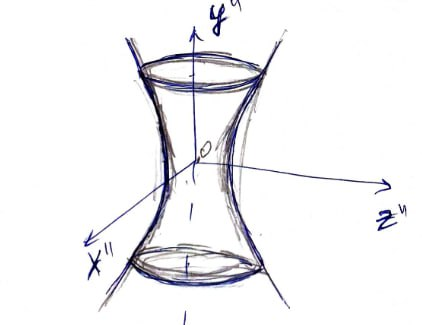
\includegraphics[width=10cm]{source/7.jpg}
\end{center}

\newpage

Итоговая замена координат выглядит следующим образом:
\[
    \begin{cases}
        x = -\d{1}{\sqrt{5}}y'' + \d{2}{\sqrt{5}}z'' \\
        y = x'' + 2                                  \\
        z = \d{2}{\sqrt{5}}y'' + \d{1}{\sqrt{5}}z''
    \end{cases}
\]

\answer{7}
\begin{itemize}
    \item Канонический вид: $2{x''}^2 - 4{y''}^2 + {z''}^2 = 3$;
    \item Поверхность: однополостный гиперболоид;
    \item Эскиз: выполнен сверху.
\end{itemize}

\newpage
\task{8}
\begin{condition}
    Линейный оператор $\varphi \colon \R^4 \to \R^4$ имеет в стандартном базисе матрицу
    \[
        \begin{pmatrix}
            1  & 3 & 3  & 1 \\
            0  & 2 & 4  & 0 \\
            0  & 0 & 2  & 0 \\
            -2 & 5 & -6 & 4
        \end{pmatrix}
    \]
    Найдите базис пространства $\R^4$, в котором матрица оператора $\varphi$ имеет жорданову форму, и укажите эту жорданову форму.
\end{condition}

Найдём значения спектра линейного оператора через характеристический многочлен. Да, может показаться страшным тот факт, что матрица порядка 4, потому предлагаю жестко успокоиться за счёт того факта, что в матрице много нулей и её определитель легко разбивается на определители поменьше. Пусть исходная матрица равна $A$, тогда:
\[
    \chi_\varphi(t) = (-1)^4 \det(A - tE) =
    \begin{vmatrix}
        1 - t & 3     & 3     & 1     \\
        0     & 2 - t & 4     & 0     \\
        0     & 0     & 2 - t & 0     \\
        -2    & 5     & -6    & 4 - t
    \end{vmatrix}
    =
    (2 - t) \cdot
    \begin{vmatrix}
        1 - t & 3     & 1     \\
        0     & 2 - t & 0     \\
        -2    & 5     & 4 - t
    \end{vmatrix}
    =
\]
\[
    = (2 - t)((1 - t)(2 - t)(4 - t) + 2(2 - t)) = (t - 2)^3(t - 3) \implies 2, 3 \in \Spec \varphi
\]

Пусть $B_t = A - tE$, узнаем количество жордановых клеток для собственного значения 2:
\[
    B_2 = A - 2E =
    \begin{pmatrix}
        -1 & 3 & 3  & 1 \\
        0  & 0 & 4  & 0 \\
        0  & 0 & 0  & 0 \\
        -2 & 5 & -6 & 2
    \end{pmatrix}
    \;
    \implies
    \;
    \rk B_2 = 3
    \;
    \implies
    \;
    d_1 = 4 -3 = 1 \text{ клетка}
\]
С учётом того, что алгебраическая кратность значения 2 равна 3 и для него определена только одна клетка - эта жорданова клетка размера 3 на 3. В таком случае, для собственного значения 3 у нас остаётся только один вариант - клетка 1 на 1, то есть для него существует собственный вектор.

Пусть $\f$ - искомый базис для линейного оператора $\varphi$, тогда его матрица примет вид:
\[
    A(\varphi, \f)
    =
    \begin{pmatrix}
        2 & 1 & 0 & 0 \\
        0 & 2 & 1 & 0 \\
        0 & 0 & 2 & 0 \\
        0 & 0 & 0 & 3
    \end{pmatrix}
    \text{ - ЖНФ}
\]

Остаётся дело за малым - предъявить базис, в котором матрица примет вид, описанный выше. Начнём с простого - найдём собственный вектор, отвечающий собственному значению 3 через ФСР:
\[
    B_3 = A - 3E =
    \begin{pmatrix}
        -2 & 3  & 3  & 1 \\
        0  & -1 & 4  & 0 \\
        0  & 0  & -1 & 0 \\
        -2 & 5  & -6 & 1
    \end{pmatrix}
    \leadsto
    \begin{pmatrix}
        1 & 0 & 0 & -\d{1}{2} \\
        0 & 1 & 0 & 0         \\
        0 & 0 & 1 & 0         \\
        0 & 0 & 0 & 0
    \end{pmatrix}
    \implies
    V_3(\varphi) =
    \langle
    \underbrace{
        \begin{pmatrix}
            \d{1}{2} \\
            0        \\
            0        \\
            1
        \end{pmatrix}
    }_{f_4}
    \rangle
    =
    \langle f_4 \rangle
\]

\newpage

Далее, для значения 2 у нас 1 клетка размера $3 \times 3$, поэтому как $f_3$ нам требуется найти такой вектор, для которого выполняется:
\[
    \vht f_3 = 3, \; f_3  \in \Ker B_2^3
\]

Вычислим матрицу $B_2^3$:
\[
    B_2^3 =
    \begin{pmatrix}
        -1 & 3 & 3  & 1 \\
        0  & 0 & 4  & 0 \\
        0  & 0 & 0  & 0 \\
        -2 & 5 & -6 & 2
    \end{pmatrix}^3
    =
    \begin{pmatrix}
        -1 & 2 & -1 & 1 \\
        0  & 0 & 0  & 0 \\
        0  & 0 & 0  & 0 \\
        -2 & 4 & -2 & 2
    \end{pmatrix}
\]

Найдём базис ядра матрицы $B_2^3$ через ФСР:
\[
    B_2^3 =
    \begin{pmatrix}
        -1 & 2 & -1 & 1 \\
        0  & 0 & 0  & 0 \\
        0  & 0 & 0  & 0 \\
        -2 & 4 & -2 & 2
    \end{pmatrix}
    \leadsto
    \begin{pmatrix}
        1 & -2 & 1 & -1 \\
        0 & 0  & 0 & 0  \\
        0 & 0  & 0 & 0  \\
        0 & 0  & 0 & 0
    \end{pmatrix}
    \implies
    \Ker B_2^3 =
    \langle
    \begin{pmatrix}
        2 \\
        1 \\
        0 \\
        0
    \end{pmatrix},\;
    \begin{pmatrix}
        -1 \\
        0  \\
        1  \\
        0
    \end{pmatrix},\;
    \begin{pmatrix}
        1 \\
        0 \\
        0 \\
        1
    \end{pmatrix}
    \rangle
\]

Промерив ручками, приходим к тому, что высоту 3 имеет только второй вектор. Берём его как $f_3$:
\[
    f_3 =
    \begin{pmatrix}
        -1 \\
        0  \\
        1  \\
        0
    \end{pmatrix}
    \;\implies\;
    f_2 = B_2f_3 =
    \begin{pmatrix}
        4 \\
        4 \\
        0 \\
        -4
    \end{pmatrix}
    \;\implies\;
    f_1 = B_2f_2 =
    \begin{pmatrix}
        4 \\
        0 \\
        0 \\
        4
    \end{pmatrix}
\]

\textbf{Обязательно:} Проверим, что набор $\f := (f_1, f_2, f_3, f_4)$ является \textit{линейно независимым}:
\[
    \begin{pmatrix}
        f_1 & f_2 & f_3 & f_4
    \end{pmatrix}
    =
    \begin{pmatrix}
        4 & 4  & -1 & \d{1}{2} \\
        0 & 4  & 0  & 0        \\
        0 & 0  & 1  & 0        \\
        4 & -4 & 0  & 1
    \end{pmatrix}
    \leadsto
    \begin{pmatrix}
        4 & 0 & -1 & \d{1}{2} \\
        0 & 4 & 0  & 0        \\
        0 & 0 & 1  & 0        \\
        0 & 0 & 0  & \d{1}{2}
    \end{pmatrix}
    \implies \f \text{ - базис в } \R^4
\]

\answer{8}
\begin{itemize}
    \item Базис
          $\f =
              (
              \begin{pmatrix}
                  4 \\
                  0 \\
                  0 \\
                  4
              \end{pmatrix},\;
              \begin{pmatrix}
                  4 \\
                  4 \\
                  0 \\
                  -4
              \end{pmatrix},\;
              \begin{pmatrix}
                  -1 \\
                  0  \\
                  1  \\
                  0
              \end{pmatrix},\;
              \begin{pmatrix}
                  \d{1}{2} \\
                  0        \\
                  0        \\
                  1
              \end{pmatrix}
              )
          $.

    \item Жорданова форма $
              A(\varphi, \f) =
              \begin{pmatrix}
                  2 & 1 & 0 & 0 \\
                  0 & 2 & 1 & 0 \\
                  0 & 0 & 2 & 0 \\
                  0 & 0 & 0 & 3
              \end{pmatrix}
          $.
\end{itemize}


\end{document}
